%!TEX root = ../book.tex
\chapter{Grasping}\label{chap:grasping}

\textsl{Grasping}\index{Grasping} is the activity for which a robot moves or manipulates and object, i.e. change its shape or pose. This is typically done by attaching an end-effector (or gripper) that is suitable to perform the task at hand.
Grasping has the interesting, and very confusing, property that it is relatively easy in practice but very complicated in theory. Consequently, this chapter describes a variety of strategies that will lead to successful grasps for a wide range of objects, but has difficulties to answer questions such as \textsl{What makes a good grasp?} or \textsl{How to find good grasps?} in any more depth than by providing simple heuristics.
In this chapter, you will learn to:
\begin{itemize}
\item how to mathematically describe grasping and where simple models reach their limitations;
\item what the properties of a gripper are that make for a good grasp in practice;
\item understand the trade-offs in a variety of grasping mechanisms.
\end{itemize}

\section{The theory of grasping}

Due to the importance of grasping in robotics, the theory behind grasping is widely investigated, with the state of the art comprehensively described in \cite{rimon2019mechanics}. However, robotics researchers still have difficulties in mathematically capturing the mechanics of grasps that are effective in practice. Therefore, rather than describing these recent developments---which are well beyond the scope of this book---we will briefly describe different approaches to model grasping and their limitations. Our goal is to provide the reader with a better understanding of the reasons for which some grasps work better than others, and what matters when designing a gripper.

In its most simple form, grasping requires immobilizing an object, at least agains the forces of gravity, by providing appropriate forces in the opposite direction, also known as \textsl{constraints}. Specifically, contact points on a robotic finger, gripper or hand are assumed to exert localized forces, thereby constraining the object sufficiently. By this, fingers essentially act as miniature robotic arms, allowing us to apply the methods and tools described in Chapters \ref{chap:locomotion}--\ref{ch:forces}.

\subsection{Friction}\index{Friction}\label{sec:grasping_friction}

In any real application, contacts between a gripper and hand are not friction-less. This is the reason grasps such as those shown in \cref{fig:idealgrasp} practically work. If there were really no friction between the fingers and the object, the object would be ejected from the hand for every grasp that is not exactly aligned with a principal axis of the cylinder in \cref{fig:idealgrasp}, left. Furthermore, even the three-finger grasp shown in \cref{fig:idealgrasp}, right, would \textsl{always} fail as there is no force constraining the object from below. Interestingly, the existance of friction makes grasping much easier in practice, yet much harder to describe mathematically.

\begin{figure}
    % 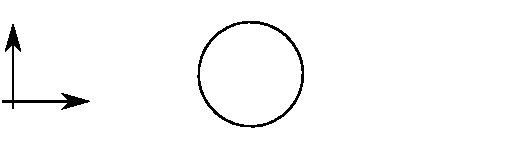
\includegraphics[width=\columnwidth]{figs/idealgrasp}
    \def\svgwidth{\textwidth}
    \import{./figs/}{idealgrasp.pdf_tex}
    \caption{Cross-section from above showing an idealized two-finger (left) and three finger (right) gripper holding a cylinder.\label{fig:idealgrasp}
   }
\end{figure}

The reason that the grasps shown in \cref{fig:idealgrasp} do work in practice is that the normal forces shown have a tangential component that is due to friction and covered by the \textsl{Coloumb's Friction law}\index{Coloumb Friction},
which states that the higher the friction coefficient of a material, the more normal force translates into tangential forces that can resist two surfaces from moving against each other.
It is governed by the equation:
\begin{equation}
F_\mathrm{t} \leq \mu\ F_\mathrm{n}.
\end{equation}

Here, $F_\mathrm{t}$  is the force of friction exerted by each surface on the other and $F_\mathrm{n}$ is the normal force; the force $F_\mathrm{t}$ acts in tangential direction to the normal force applied by, e.g., a fingertip; $\mu$ is a coefficient of friction that can be measured empirically---intuitively, $\mu$ is low for glass on glass and high for rubber on wood.
We are therefore interested in designing grippers with high friction coefficients to avoid objects from slipping.

\begin{figure}
    % 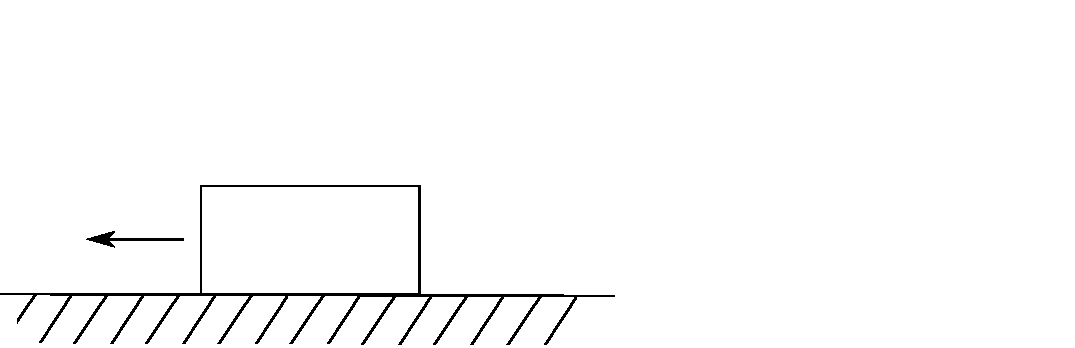
\includegraphics[width=\columnwidth]{figs/coulombfriction}
    \def\svgwidth{\textwidth}
    \import{./figs/}{coulombfriction.pdf_tex}
    \caption{Left: Coloumb friction relates normal to tangential reaction forces that are required to overcome friction, here shown for rightwards motion. Right: Friction cone for point forces. As long as the force is within the cone cone, the finger will not slip.}\label{fig:coulombfriction}
\end{figure}

When do objects slip? Let's analyze the problem via \cref{fig:coulombfriction}. Say we have a fingertip pressing down on a surface in any orientation. There will be a force normal to the surface $F_\mathrm{n}$, which defines the tangential force $F_\mathrm{t}$ in any direction. Sweeping the tangential force around the normal force creates a cone with an opening angle of:
\begin{equation}
\alpha=2tan^{-1}\mu,
\end{equation}
see \cite[p. 57]{rimon2019mechanics} for a derivation.
If the net force on the object is not within this cone, the object slips.  This becomes more intuitive when thinking about how different values of $\mu$ affect the shape of this cone. If $\mu$ is high, the cone will be relatively wide, letting the object ``accept'' forces from many different directions without slipping. If $\mu$ is low, the cone will be relatively narrow, requiring the force to be normal to the object's surface to prevent slippage.

Importantly, as detailed in \cref{ch:forces}, a force applied to a rigid body will exert both a 3D force as well as a 3D moment to the body's center of gravity; this quantity is called a \textsl{wrench}\index{Wrench}---see \cref{eq:wrench:force,eq:wrench:moment}. If we consider all the possible wrenches that we can apply to a rigid body without having the end-effector slip to form a space (namely the cone described earlier for a single finger), we can talk about the \textsl{grasping wrench space}\index{Grasping wrench space}, which is the corresponding space of all suitable wrenches.
%
Knowing the relation between normal and tangential reaction forces can help in designing grippers that are more likely to successfully grasp an object than others, as well as when planning suitable grasp for objects with known friction.

%In summary: we can use Coloumb's law of friction to determine the direction of forces that we can apply to a certain contact point without that the object slips. These forces translate into wrenches to the object's center of gravity. A grasp fits a certain task if the wrenches that would fulfill the task can be effectuated without slip. The less force is waisted to overcome slip, the better is the grasp.

\subsection{Multiple contacts and deformation}\label{sec:grasping_deformation}

In practice, no force will ever be applied at a single point only; rather, a force will be distributed over an area, either due to the size of the finger pad itself or due to the contact area deforming under pressure.
Even the smallest contact area that is not a point in the mathematical sense will add constraints on torque, which will translate to constraints in additional dimensions and therefore further stabilization of the grasp. This is illustrated in \cref{fig:contactarea}.
A single point of contact (\cref{fig:contactarea}, left) allows the object to easily pivot around it; however, by increasing the contact area we are able to costrain the rotational degree of freedom, thus reducing the available DoFs for the object to only its translational component.
It is therefore desirable to grasp an object with a contact area that is as large as possible. Importantly, since as surfaces are not ideally flat, this extension of contact are is only possible in practice the contact area is deformable---see \cref{fig:contactarea}, right. Lastly, a large contact area will also increase friction, which as detailed in \cref{sec:grasping_friction} is a desirable property for grasping.

\begin{figure}
    % 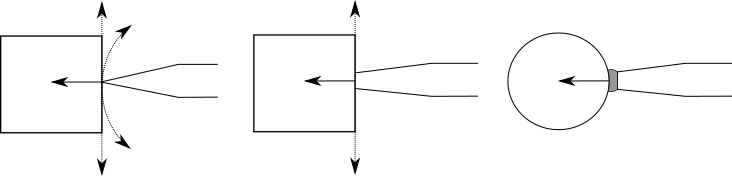
\includegraphics[width=\columnwidth]{figs/graspingcontacts}
    \def\svgwidth{\textwidth}
    \import{./figs/}{graspingcontacts.pdf_tex}
    \caption{From left to right: ideal force exerted via a single point of contact, forces exerted via an area of contact, contact area increasing due to pressure and conforming with the surface. Remaining degrees of freedom are indicated by dotted lines. \td{Nikolaus, which dotted lines? I don't see any} \label{fig:contactarea}}
\end{figure}

Consequently, using metal jaws or rigid fingers is seldom successful in practice. Instead, rubber pads are used to increase force closure by conforming around the object. As the rubber is flexible, however, the grasp is not completely stabilizing the object and it may still be able to move within the grasp; this might not be desirable for precise manipulation tasks such as picking up a nut and trying to mount it on a screw. Mathematically, this introduces additional complications into the grasp model in the form of elasticity introduced in the object--robot dynamics; in simple terms, soft/flexible pads are the equivalent of a spring, increasing uncertainty in its dynamics.

\subsection{Suction}

A highly effective method for grasping is using suction. Here, a suction cup is pressed against an object, using a vacuum applied by a pump to suck the object against the cup. Instead of exerting forces against the object, which always requires at least one antipodal force (or multiple forces that are distributed such that the object remains in equilibrium) to create a constraint, suction only requires one point of contact. The rim of the suction cup provides both friction and multiple contact points to prevent the object from slipping and further constraining the object beyond the normal force applied by the vacuum.
Requiring only a single area of contact is a tremendous advantage from a planning perspective as only one area on an object needs to be identified, whereas other grasping approaches need to always identify two areas and coordinate motion to reach them.
It is worth noting that suction using multiple suction cups on custom-made rigs to grasp large parts such as car doors is very popular in the car industry, but it generally relies on pre-programmed trajectories and little to no autonomy---which is not a focus of this book.

The soft nature of the suction cup provides the ability for the rim to conform to the object, but makes suction impractical for objects that do not have any flat surfaces or and that expose holes to the gripper---for example, objects stored in a net. The elasticity of the rim also makes it difficult to further manipulate the object as all forces applied by the robot will need to be transferred via a spring-like elastic material. Finally, suction requires a vacuum pump that is able to generate sufficient force to lift an object, limiting the maximum weight of objects suitable for suction by a single suction cup in practice.

\section{Simple grasping mechanisms}\label{sec:simplegrasp}

Understanding why grasping actually works---namely, via friction (\cref{sec:grasping_friction}) and increasing contact area due to deformation (\cref{sec:grasping_deformation}), allows us to select grasping mechanism that are characterized by the following properties: 1) they are able to successfully grasp a wide range of objects, 2) they are simple to construct, and 3) they are easy to control.
Here, properties of interest are the range of possible object sizes, the maximum weight of an object, and how fragile objects can possibly be. Object dimensions are directly dependent on the gripper kinematics such as minimum and maximum aperture, whereas the maximum weight is given by the torque the mechanism can exert as well as the number of contacts and their friction parameters. Whether a gripper can handle fragile objects is a function of how well this torque can be measured and controlled.

\subsection{1-DoF scissor-like gripper}

One of the simplest grippers is a simple one degree-of-freedom claw, which is a popular design in the prosthetic community, and has been refined for centuries. Actuated by a string mounted to a person's shoulder, or more recently by electric motors controlled via muscle activity in the lower arm, this simple mechanism enables the wearer to perform a wide range of everyday activities. Indeed, an off-the-shelf prosthetic hand has been shown to perform a large variety of grasping and manipulation tasks when compared with other robotic hands in a tele-operation scenario, only limited by its ability to conform to specific kinematic constraints such as operating scissors \cite{patel2016manipulation}.

\begin{figure}
    % 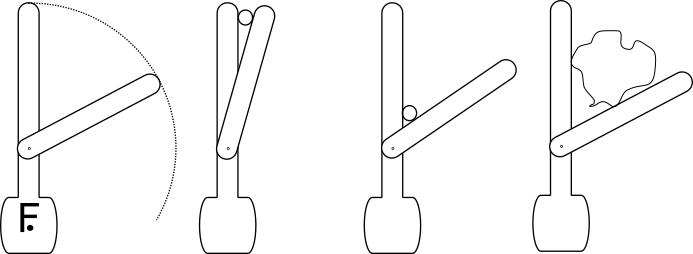
\includegraphics[width=\columnwidth]{figs/gripper-1-dof}
    \def\svgwidth{\textwidth}
    \import{./figs/}{gripper-1-dof.pdf_tex}
    \caption{Simple 1-DoF grasping mechanism that relies on friction to grasp objects with a wide variety of sizes (center, right). The mechanism has only one moving part that presses the object against a passive finger.}\label{fig:gripper-1-dof}
\end{figure}

A simple design is shown in \cref{fig:gripper-1-dof} and consists of an active finger that presses an object against a passive finger, with both fingers often shaped as a hook. As should be clear by now, such a design can only work by relying on friction, which makes it not very common in traditional robotics.

The key advantage of this mechanism is because it allows for very simple control strategies to operate it: use the passive finger to make contact with the object, then use the active finger to close the grasp.
The event ``make contact" can either be detected by measuring the force acting at the wrist and looking for abrupt changes in such force or using a tactile sensor on the finger with which contact is made. This approach can therefore lead to robust grasps with a minimum of sensing required. A disadvantage of this mechanism is that its function relies exclusively on friction, possibly ejecting away objects from its grasp if friction is not sufficient or the object is in an otherwise sub-optimal conformation. Unlike most other mechanisms, it is also impossible to use the finger position to infer the width of an object, which is illustrated by the illustrations in \cref{fig:gripper-1-dof}, center.

The mechanism shown in \cref{fig:gripper-1-dof} can be actuated in many different ways, for example by attaching a servo motor directly to the active finger, using a shape-memory alloy wire via a suitable lever arm, or a pneumatic piston or balloon.

\subsection{Parallel jaw}

The most common industrial gripper mechanism is the two-finger parallel jaw gripper. It operates by squeezing an object between its two parallel jaws, which are usually driven by a single actuator and therefore move in concert. Parallel jaw grippers usually yield more contact area than a scissor-like 1-DoF gripper, but suffer from a smaller range of motion.

\begin{figure}
\centering
    % 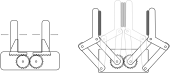
\includegraphics[width=\columnwidth]{figs/gripper-2-dof}
    \def\svgwidth{\textwidth}
    \import{./figs/}{gripper-2-dof.pdf_tex}
    \caption{Left: Parallel jaw gripper driven by a single actuator via a system of coupled gears. Right: 4-bar linkage parallel jaw gripper.}\label{fig:paralleljaw}
\end{figure}

\cref{fig:paralleljaw}, left, shows a minimalist implementation of a parallel jaw gripper that can be actuated by a single servo motor, driving two rack gears to which the gripper jaws are mounted. While using gears on racks is unusual in an industrial design---the gripper jaws typically travel on threads actuated by worm gears or are attached to a pneumatic piston---this drawing illustrates the relationship between the range of motion of the gripper jaws, the length of the mechanism it is sliding on (here a rack gear), and the resulting body size. In order for this design to fully close, the two rack gears must be mounted at an offset in order to slide against each other. Constraints like this often make the gripper body twice as wide as the maximum aperture, making it difficult for the robot to enter tight areas. The mechanical design also affects the speed at which a gripper can operate. Pneumatic grippers, where air pressure coming in on either end of the piston can drive the gripper into an ``open'' or ``close'' position very quickly (2-3 times per second), cannot be controlled accurately. Electric mechanisms instead trade-off accuracy and torque with speed (i.e. more accuracy but at lower speed).

The control strategy for parallel jaw grippers requires an accurate pose estimation of the object of interest and a precise positioning the gripper so that the object is right in the center of the two jaws. Note that force-closure with a static object, such as a screw mounted to a structure, requires both jaws to make contact with the object at the same time, thereby imposing high accuracy requirements on both object detection and robot motion. Here, compliance can help, allowing the gripper to adjust its pose to the object. This can be accomplished by either measuring forces in the wrist and moving the gripper to minimize lateral forces or a compliant mounting mechanism or structure, such as a robot equipped with series-elastic or pneumatic actuators. An alternative approach is to actuate both gripper jaws independently, as seen below.

\subsection{4-bar linkage parallel gripper}

A parallel jaw mechanism with a larger range of motion can be accomplished using two 4-bar linkages---see \cref{fig:paralleljaw}, right. In a 4-bar linkage, rotation of the motor is translated into straight translation of the fingers. This is accomplished by two pairs of parallel bars of equal lengths. In \cref{fig:paralleljaw}, right, one of the four bars is not moving and substituted by the gripper body, to which two of the bars are mounted \td{nikolaus I don't understand this sentence. It seems important though}. Interestingly, both pairs remain parallel as one of the bars is rotating, resulting in the two gripper jaws remaining parallel to each other. This is best understood by inspecting \cref{fig:paralleljaw} and comparing the two positions the left jaw can be in.

The drawback of this design is that closing the gripper also results in a forward motion. This requires approaching an object from different distances, depending on its width. Other than this, the control strategy is the same as for the parallel jaw gripper, requiring an accurate estimate of the object's pose. Also here, adding compliance or independent actuation of each jaw can help resolving accuracy problems.

\subsection{Multi-fingered hands}

Grippers with more than two fingers/jaws are rarely used in industrial practice. One common use case is grasping cylindrical objects from above, for which three-fingered hands, such as the one shown in \cref{fig:idealgrasp}, right, are best suited. However, in most other cases three fingers are not an advantage, and might even be a hindrance!
For example, it is difficult to perform simple pinching grasps with three fingers. This has led to designs in which two of the fingers are reconfigurable from performing an inwards motion to behave identical to a parallel jaw gripper, while the third finger is stored in a safe position. In addition to mechanical complexity, such an approach requires also additional planning steps.

How many grasps are possible and how many possible grasps are needed to grasp every possible object remains a difficult theoretical problem (which is further complicated by the fact that successful grasping often happens at the boundary of what is mathematically tractable). Generally, we can say however that additional fingers---such as in the human hand---provide additional redundancy, which allows grasping and manipulating (see Section \ref{chap:manipulation}) the same object in many different ways, including manipulating the object within the hand, that is without intermittent placement or handing it over to another gripper.

\section*{Take-home lessons}
\begin{itemize}
\item Making a good gripper requires to take advantage of compliance and friction in a way that still eludes mathematical analysis, making gripper design an experimental process.
\item Successfully grasping an item does not necessarily mean that the robot will also be able to successfully manipulate that item. Designing a grasping mechanism therefore requires to understand the entire task, from grasping to placing or otherwise manipulating the item. 
\item Simple mechanisms such as suction or two finger grippers are sufficient for most grasping and manipulation tasks, but are not suitable for in-hand manipulation, which---for the large part---remains an open research challenge.
\end{itemize}


\section*{Exercises}\small
\begin{enumerate}
\item Think about at least three mechanisms to realize a parallel jaw gripper. How does the minimum and maximum aperture of the gripper relate to the gripper width for each of these designs?
\item Think about at least three mechanisms to actuate a four-bar linkage. Which of these will keep the payload inside the gripper during power failure?
\item Derive an equation for the distance of the fingertip from the gripper base in a 4-bar linkage gripper as a function of the gripper opening width. Use appropriate parameters for all unknown parameters.
\item A powerful mechanism to grasp is to evacuate the air from a bag of coffee beans after conforming around an object. Describe what happens here using language from this chapter.
\item Design a grasping system to pick up the bare metal of a car door for assembly in an automated manufacturing line. Which design ensures maximal accuracy in placing the part? 
\end{enumerate}\normalsize
